% DAG phụ thuộc dự báo trong cùng repeat; shared-input relation vẽ riêng.
\documentclass[10pt]{article}
\usepackage[T1]{fontenc}
\usepackage{lmodern}
\usepackage[paperwidth=180mm,paperheight=155mm,margin=4mm]{geometry}
\usepackage{tikz}
\usetikzlibrary{arrows.meta}
\pagestyle{empty}
\setlength{\parindent}{0pt}
\definecolor{ink}{HTML}{1F3445}
\definecolor{teal}{HTML}{126B80}
\begin{document}
\centering
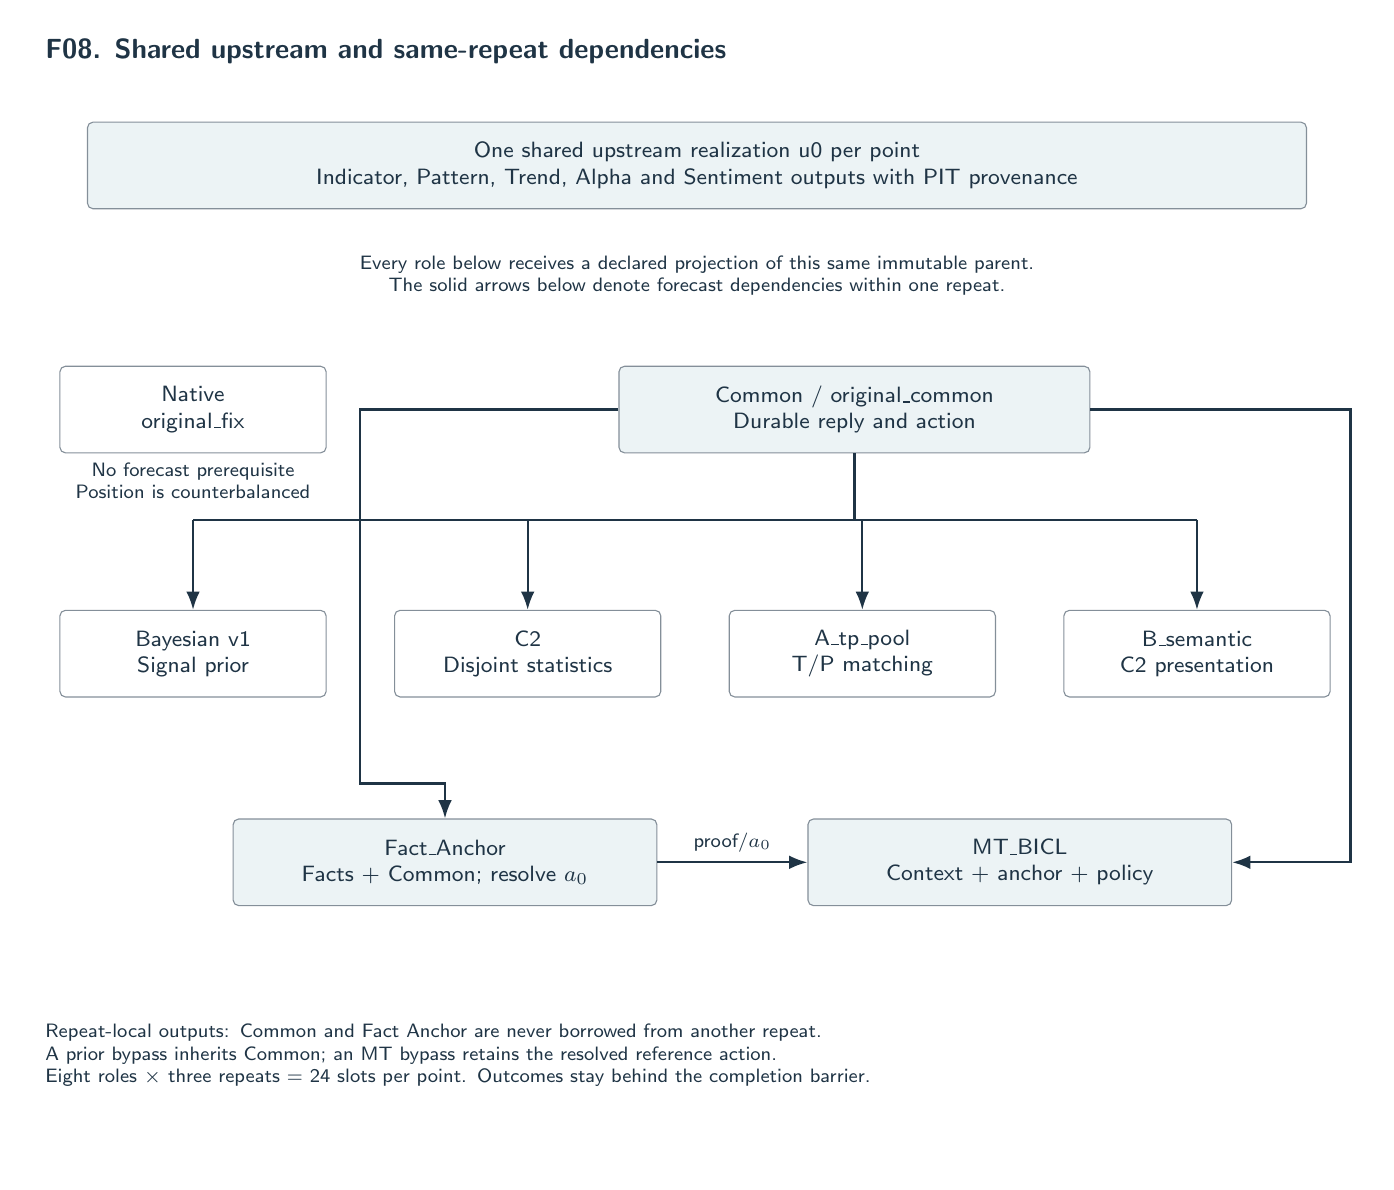
\begin{tikzpicture}[x=1cm,y=1cm,>=Latex,font=\sffamily\footnotesize,text=ink,
 box/.style={draw=ink!55,rounded corners=2pt,align=center,text width=3.1cm,minimum height=1.1cm,inner sep=4pt},
 flow/.style={->,thick,draw=ink}]
\path[use as bounding box] (0,0) rectangle (17,14.4);
\node[anchor=west,font=\sffamily\bfseries] at (.1,14.1) {F08. Shared upstream and same-repeat dependencies};
\node[box,text width=15.2cm,fill=teal!8] (shared) at (8.5,12.65)
 {One shared upstream realization u0 per point\\Indicator, Pattern, Trend, Alpha and Sentiment outputs with PIT provenance};
\node[align=center,text width=16cm,font=\sffamily\scriptsize] at (8.5,11.25)
 {Every role below receives a declared projection of this same immutable parent.\\The solid arrows below denote forecast dependencies within one repeat.};
\node[box] (native) at (2.1,9.55) {Native\\original\_fix};
\node[box,fill=teal!8,text width=5.7cm] (common) at (10.5,9.55) {Common / original\_common\\Durable reply and action};
\node[font=\sffamily\scriptsize,align=center,text width=3.2cm] at (2.1,8.65) {No forecast prerequisite\\Position is counterbalanced};
\node[box] (v1) at (2.1,6.45) {Bayesian v1\\Signal prior};
\node[box] (c2) at (6.35,6.45) {C2\\Disjoint statistics};
\node[box] (a) at (10.6,6.45) {A\_tp\_pool\\T/P matching};
\node[box] (b) at (14.85,6.45) {B\_semantic\\C2 presentation};
\coordinate (bus) at (10.5,8.15);
\draw[thick,draw=ink] (common.south) -- (bus) -- (2.1,8.15);
\draw[thick,draw=ink] (bus) -- (14.85,8.15);
\foreach \node in {v1,c2,a,b} {\draw[flow] (\node.north |- bus) -- (\node.north);}
\node[box,fill=teal!8,text width=5.1cm] (anchor) at (5.3,3.8) {Fact\_Anchor\\Facts + Common; resolve $a_0$};
\node[box,fill=teal!8,text width=5.1cm] (mt) at (12.6,3.8) {MT\_BICL\\Context + anchor + policy};
\draw[flow] (common.west) -- (4.225,9.55) -- (4.225,4.8) -- (5.3,4.8) -- (anchor.north);
\draw[flow] (common.east) -- (16.8,9.55) -- (16.8,3.8) -- (mt.east);
\draw[flow] (anchor.east) -- node[above,font=\sffamily\scriptsize] {proof/$a_0$} (mt.west);
\node[align=left,text width=16.3cm,font=\sffamily\scriptsize,anchor=west] at (.1,1.35)
 {Repeat-local outputs: Common and Fact Anchor are never borrowed from another repeat.\\A prior bypass inherits Common; an MT bypass retains the resolved reference action.\\Eight roles $\times$ three repeats = 24 slots per point. Outcomes stay behind the completion barrier.};
\end{tikzpicture}
\end{document}
